\section{其它}
%官方要求：除了机械、硬件、软件、算法之外的研发投入说明，比如：工业设计、UI交互开发。
\subsection{实时性}
我们为 Linux 内核打上 PREEMPT\_RT\cite{RTwiki60:online} 补丁。如  \figref {fig:rt_test}  所示，我们使用了\lstinline{cyclictest} 进行了500000个循环的测试，打补丁后的最大延迟有三个数量级的下降，且频次更加靠左（延迟更小），更加集中，可见实时性有了较大的提升，经过CAN回环和实车等测试，满足RM需求。
\begin{figure}[hbt!]
   \centering
   \subfigure[未打实时补丁]{
      \centering
       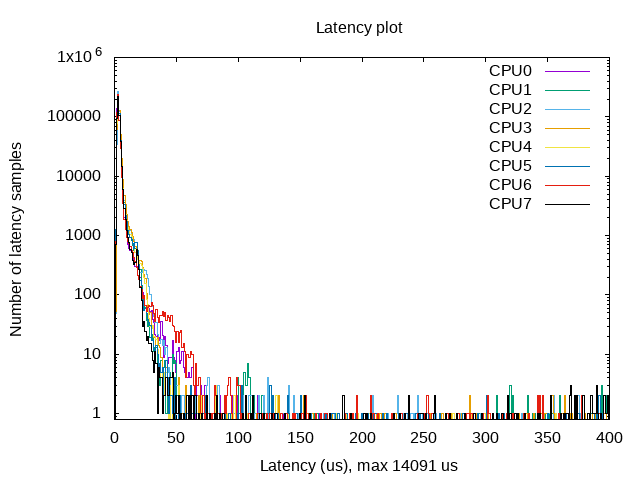
\includegraphics[width=0.45\columnwidth]{figure/设计方案/软件设计/rt_test0.png}
   }
   \subfigure[已打实时补丁]{
       \centering
       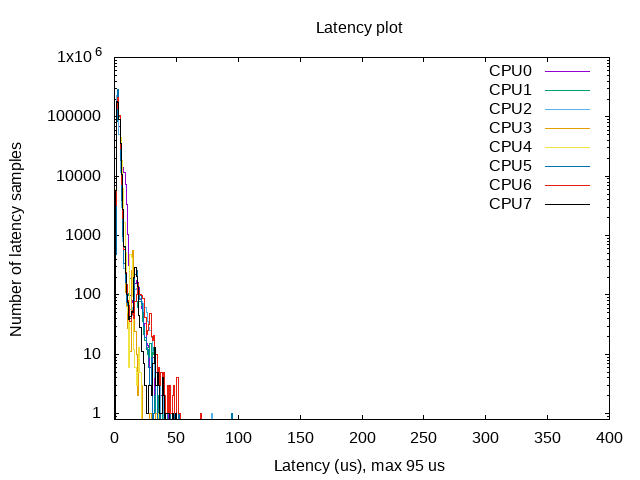
\includegraphics[width=0.45\columnwidth]{figure/设计方案/软件设计//rt_test1.png}
   }
   \caption{在Intel NUC 上在压力下的实时性测试结果，横轴为延迟大小，纵轴为频次}
    \label{fig:rt_test}
\end{figure}
\subsection{通过裁判系统数据的读取对机器人控制的优化}
\subsubsection{功能说明}
控制程序通过串口读取裁判系统数据使得机器人的各模块参数与比赛时的性能体系或是时间节点相匹配，或是通过裁判系统的数据对超级电容中的电流采样模块所进行校准。

\subsubsection{各模块参数与性能体系的匹配}

\begin{itemize}
    \item \textbf{底盘模块}：比赛阶段，决策层收到裁判系统中关于底盘上限功率的数据后，将数据发送到chassis controller中，chassis controller根据上限功率算出底盘电机的最大输出力矩，并作为PID的输入，从而达到功率限制的目的；
    \item \textbf{发射模块}：比赛阶段，决策层收到裁判系统中关于42mm弹丸初速度上限的数据后，将指令发送到shooter controller中，shooter controller根据$\qty{42}{\mm}$弹丸初速度上限读取配置文件中对应的摩擦轮转速，并作为PID的输入，从而保证$\qty{42}{\mm}$弹丸初速度不超过上限。
    \item \textbf{视觉模块}：比赛阶段，视觉模块根据裁判系统中的敌方颜色，设定识别灯条的颜色。
\end{itemize}

\subsubsection{校准超级电容的电流采样模块}
三分钟准备阶段，超级电容的主控开始大功率充电，同时通过裁判系统数据中的底盘实时功率，对电流采样模块反馈的数据进行校准，保证比赛阶段电流采样模块反馈的数据的准确性。


\subsection{调试工具}
rqt是一个基于Qt的框架，用于ROS的GUI开发。本团队利用各种插件组合成自定义界面，写成配置文件后日常调试中使用。下面对该自定义配置界面进行介绍。

\subsubsection{Home}
本界面如 \figref {fig:rqt_home}所示。界面左侧用于显示机器人的姿态，通过RVIZ插件，在日常调试中常用于观察机器人的tf坐标系以及机器人模型是否正确。界面右侧通过订阅相应话题，可以实时观察从摄像头传回的图像。右下方加入了动态调参的插件，便于调整参数。在日常调试中常用于调试视觉参数。
\begin{figure}[htpb]
   \centering
  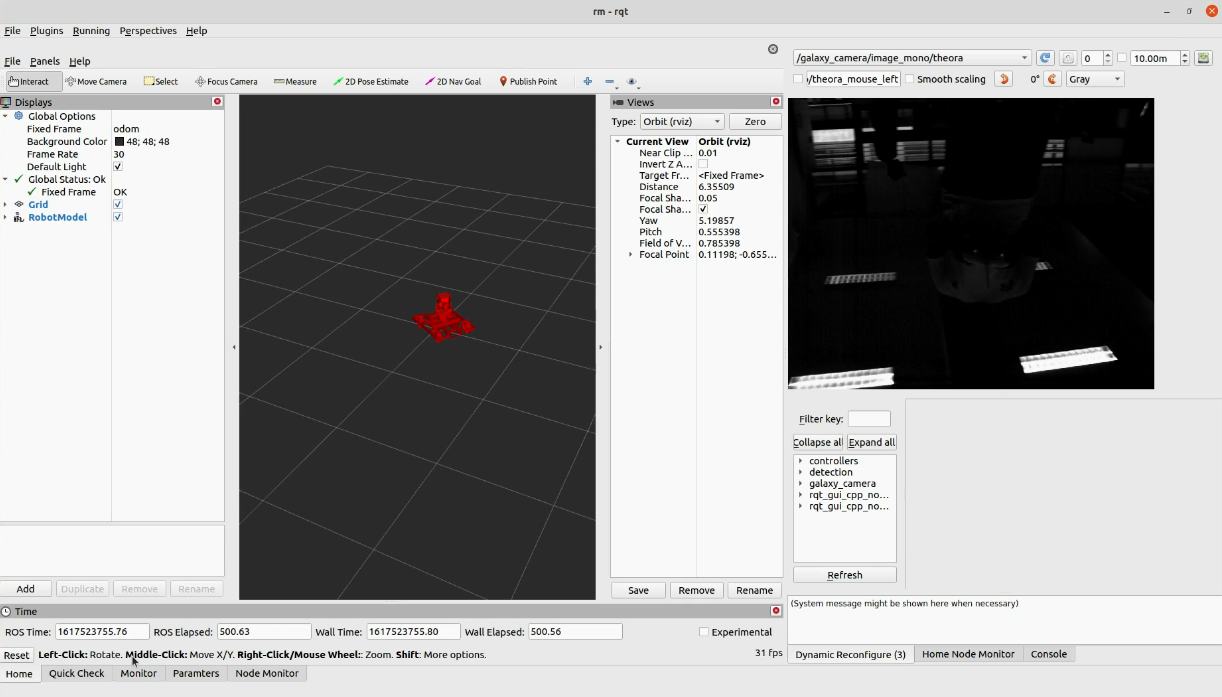
\includegraphics[width=0.8\columnwidth]{figure/设计方案/软件设计/rqt_home.png}
    \caption{Home界面}
    \label{fig:rqt_home}
\end{figure}

\subsubsection{Quick Check}
本界面用于快速检查代码运行状态，如 \figref {fig:rqt_quickcheck}所示。界面左侧显示各个节点的CPU和内存占用情况，以及输出的各项信息。界面右侧可以看到整个tf树的结构以及各个节点之间的通讯关系。在日常调试中通常用于观察输出的调试信息或者检查某个节点有没有在运行。

\begin{figure}[htpb]
    \centering
    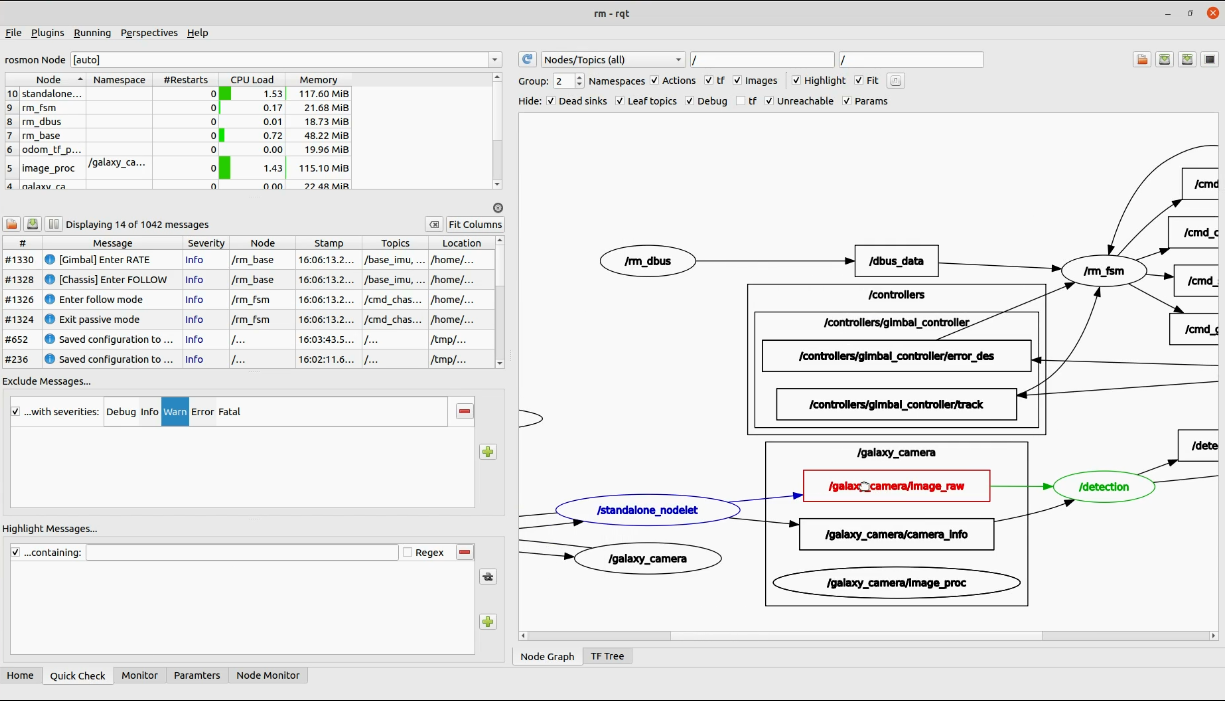
\includegraphics[width=0.8\columnwidth]{figure/设计方案/软件设计/rqt_quickcheck.png}
    \caption{Quick Check界面}
    \label{fig:rqt_quickcheck}
\end{figure}


\subsubsection{Monitor}
本界面显示机器人读取到的各项信息。分为4个子界面。分别是\textbf{Joint, Imu, Referee, Topic}

\paragraph{Joint}
本界面用于显示电机的速度和力矩，如 \figref {fig:rqt_monitor_joint}所示。通过rqt\_multiplot插件绘制出电机的速度或力矩图像。使用过程中，不仅可以对单个电机的数据进行清空或记录，也可以对全部电机的数据同时清空或记录，还可以单独放大某个电机的图像，方便观察。

\begin{figure}[!htbp]
    \centering
    \subfigure[多电机]{
        \centering
        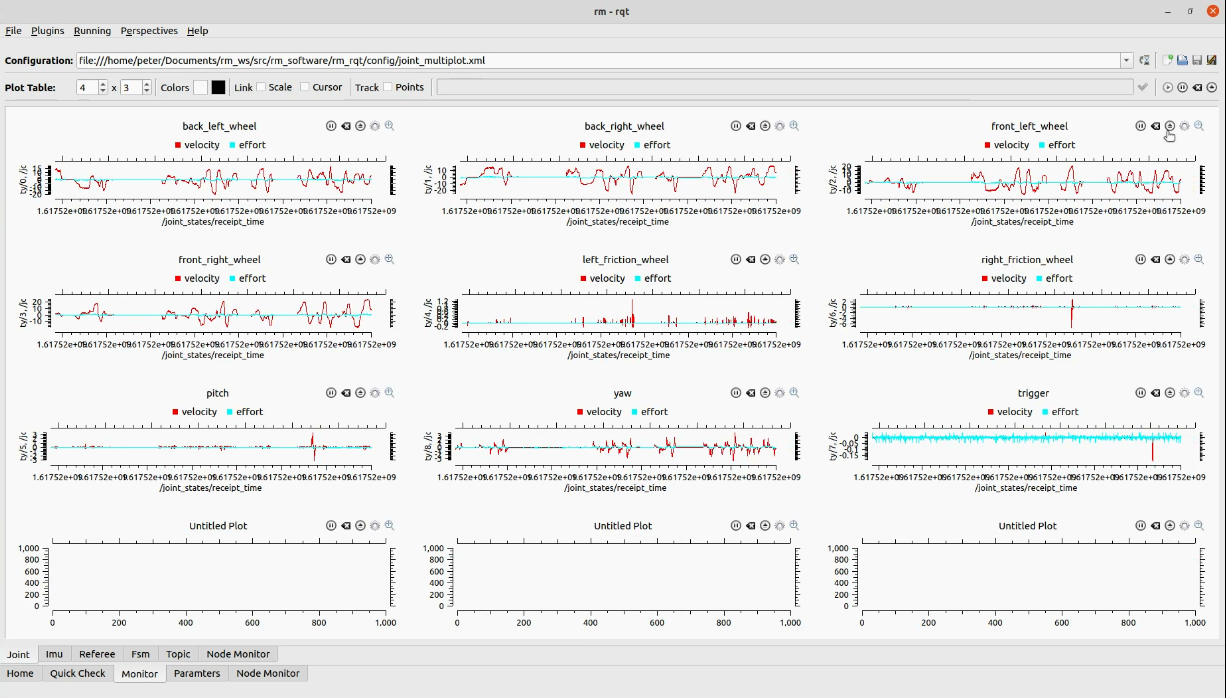
\includegraphics[width=0.7\columnwidth]{figure/设计方案/软件设计/rqt_monitor_joint.png}
    }
    \subfigure[单电机]{
        \centering
        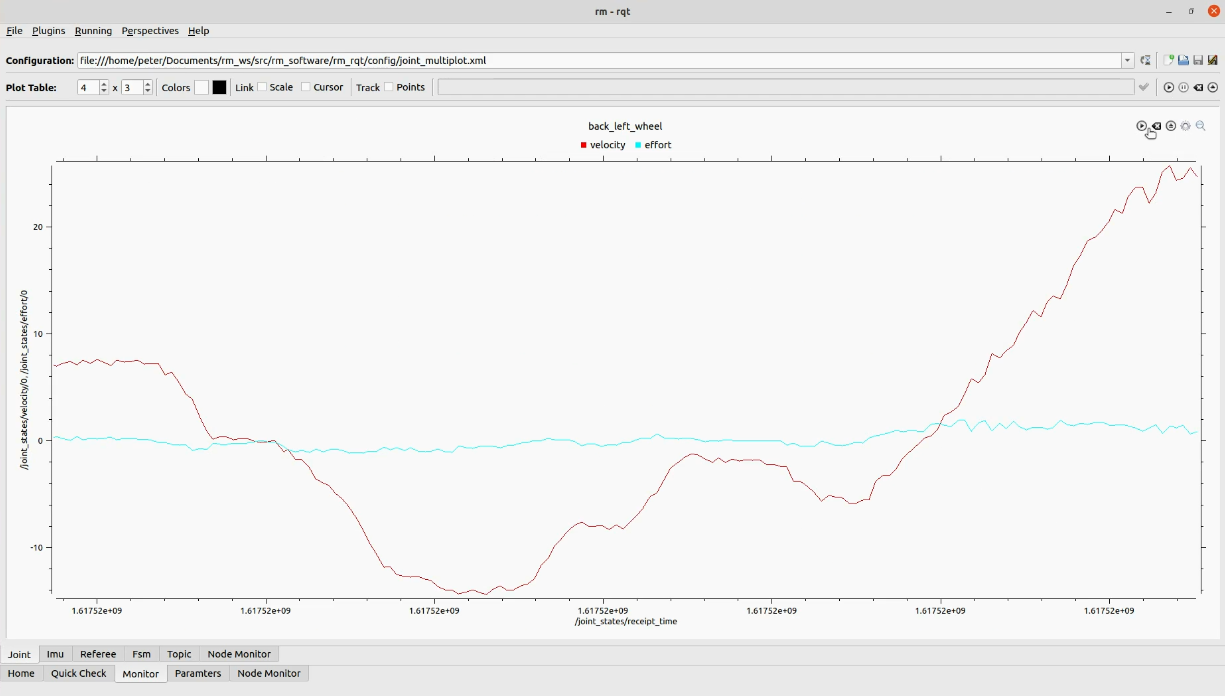
\includegraphics[width=0.7\columnwidth]{figure/设计方案/软件设计/rqt_monitor_joint_single.png}
    }
    \caption{Joint界面 \label{fig:rqt_monitor_joint}}
\end{figure}

\paragraph{Imu}
本界面用于显示IMU返回的数据，同样也是通过rqt\_multiplot插件绘制出IMU返回的姿态信息。功能与Joint界面类似，此处不再重复说明。

\paragraph{Referee}
本界面用于显示裁判系统的各项信息，如 \figref {fig:rqt_monitor_referee}所示。同样也是通过rqt\_multiplot插件绘制出裁判系统数据图像。在实际调试中常用于调试底盘功率限制或枪口热量限制。

\begin{figure}[htpb]
    \centering
    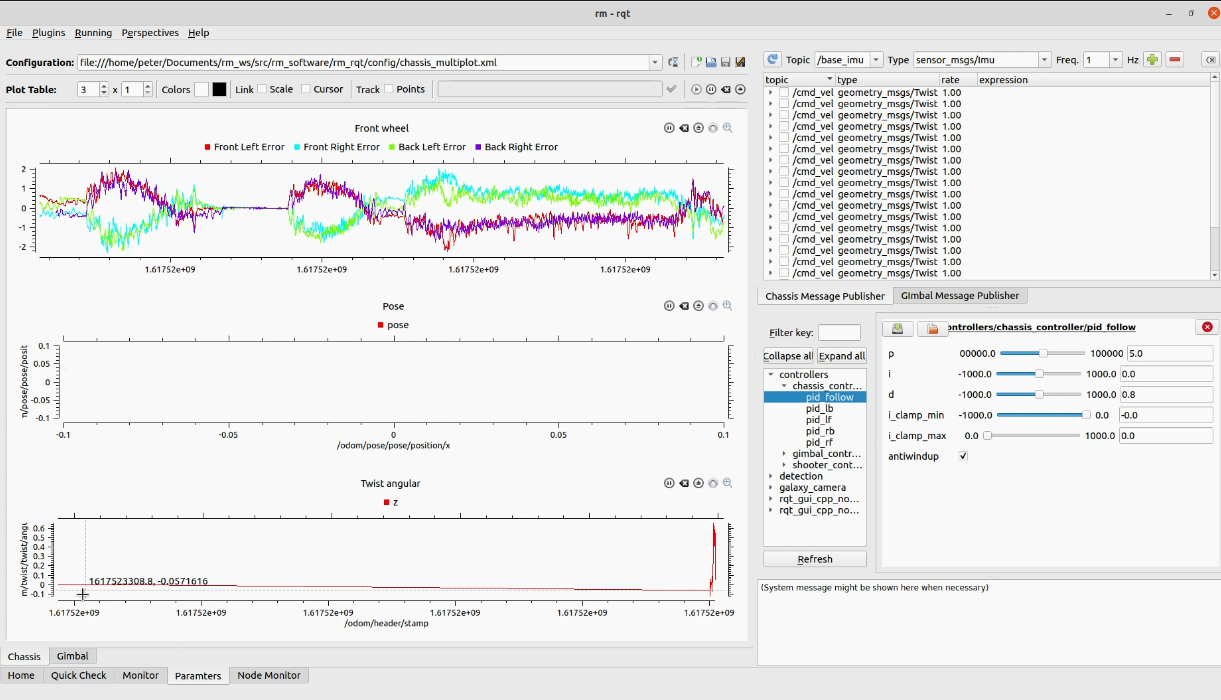
\includegraphics[width=0.7\columnwidth]{figure/设计方案/软件设计/rqt_parameter_chassis.png}
    \caption{Referee界面}
    \label{fig:rqt_monitor_referee}
\end{figure}

\paragraph{Topic}
本界面用于显示机器人运行时所有话题下的消息，如 \figref {fig:rqt_monitor_topic}所示。通过勾选相应话题即可读取到该话题上消息的发送频率、消息的值以及消息类型等等。在实际调试中常用于判断问题出现在哪个包。
\begin{figure}[htpb]
    \centering
    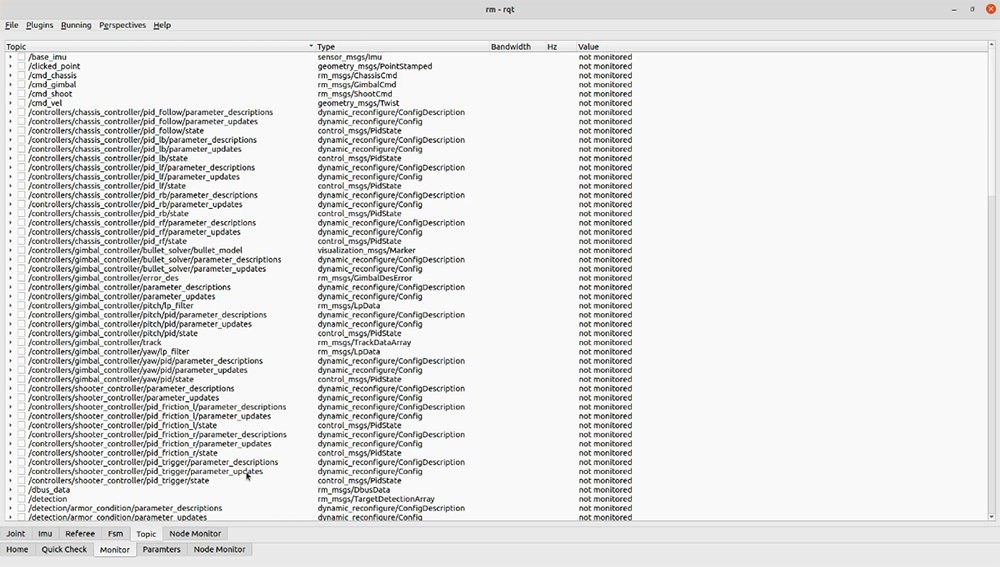
\includegraphics[width=0.7\columnwidth]{figure/设计方案/软件设计/rqt_monitor_topic.jpg}
    \caption{Topic界面}
    \label{fig:rqt_monitor_topic}
\end{figure}

\subsubsection{Parameters}
本界面用于调试控制器参数。分为2个子界面，分别是\textbf{Chassis，Gimbal}
\paragraph{Chassis}
本页面用于调试底盘控制器的参数，如 \figref {fig:rqt_parameter_chassis}所示。在界面左侧可以观察到底盘电机的各项数据，如误差、姿态等，也可以手动添加其他电机信息。界面右侧的上方可以直接向底盘订阅的话题发送命令消息；下方则可以对底盘PID参数进行动态调整，方便调试。
\begin{figure}[htpb]
    \centering
    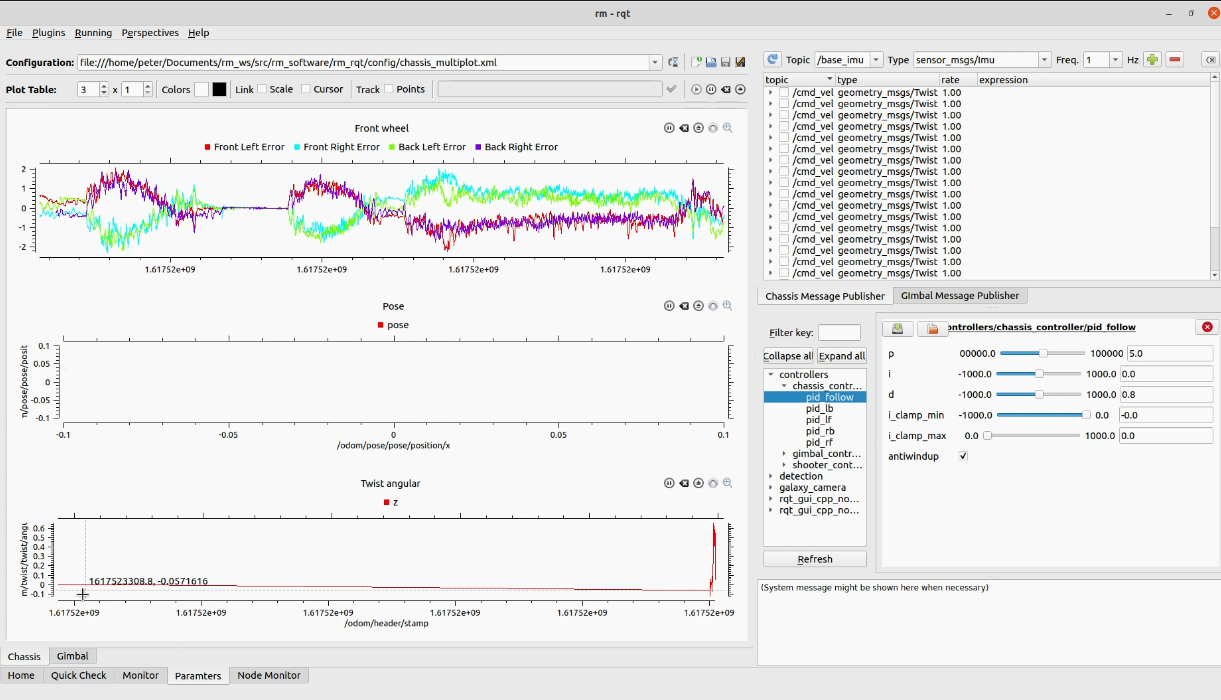
\includegraphics[width=0.7\columnwidth]{figure/设计方案/软件设计/rqt_parameter_chassis.png}
    \caption{Chassis界面}
    \label{fig:rqt_parameter_chassis}
\end{figure}

\paragraph{Gimbal}
本页面用于调试云台控制器的参数，如 \figref {fig:rqt_parameter_gimbal}所示。具体功能与\textbf{Chassis}界面类似，在此不再重复说明。
\begin{figure}[htpb]
    \centering
   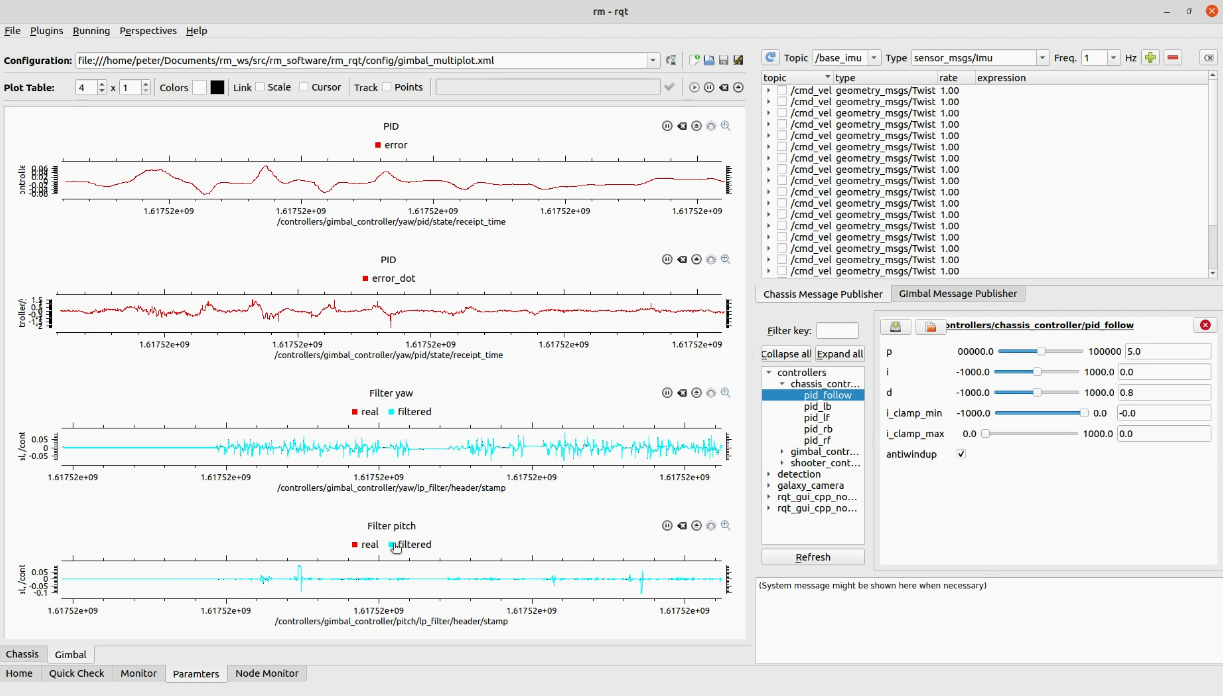
\includegraphics[width=0.7\columnwidth]{figure/设计方案/软件设计/rqt_parameter_gimbal.png}
    \caption{Gimbal界面}
    \label{fig:rqt_parameter_gimbal}
\end{figure}

\paragraph{Shooter}
本页面用于调试发射控制器的参数。具体功能与\textbf{Chassis}界面类似，在此不再重复说明。

\subsection{手眼标定与联合标定}
\subsubsection{手眼标定}
手眼标定是指标定相机坐标系与机器人坐标系的转换关系，可分为Eye-in-Hand和Eye-to-Hand。在RoboMaster中，需要确定相机与云台的精确的相对位置关系，这样才能提高自瞄的准确度。如果相机坐标系与机器人坐标系的转换关系不准确，那么程序对目标在世界坐标系的位姿估计实际上是不准确的。在urdf中，相机坐标系与机器人坐标系的转换关系是根据图纸中的数据来确定的，但由于加工与装配的误差，urdf中的这一转换关系与实际机器人中的存在误差。为了精确确定相机坐标系与云台坐标系的转换矩阵，我们使用第三方的ROS软件包 easy\_handeye\cite{easy_handeye:online} 来进行手眼标定。

\begin{figure}[hbt!]
    \centering
    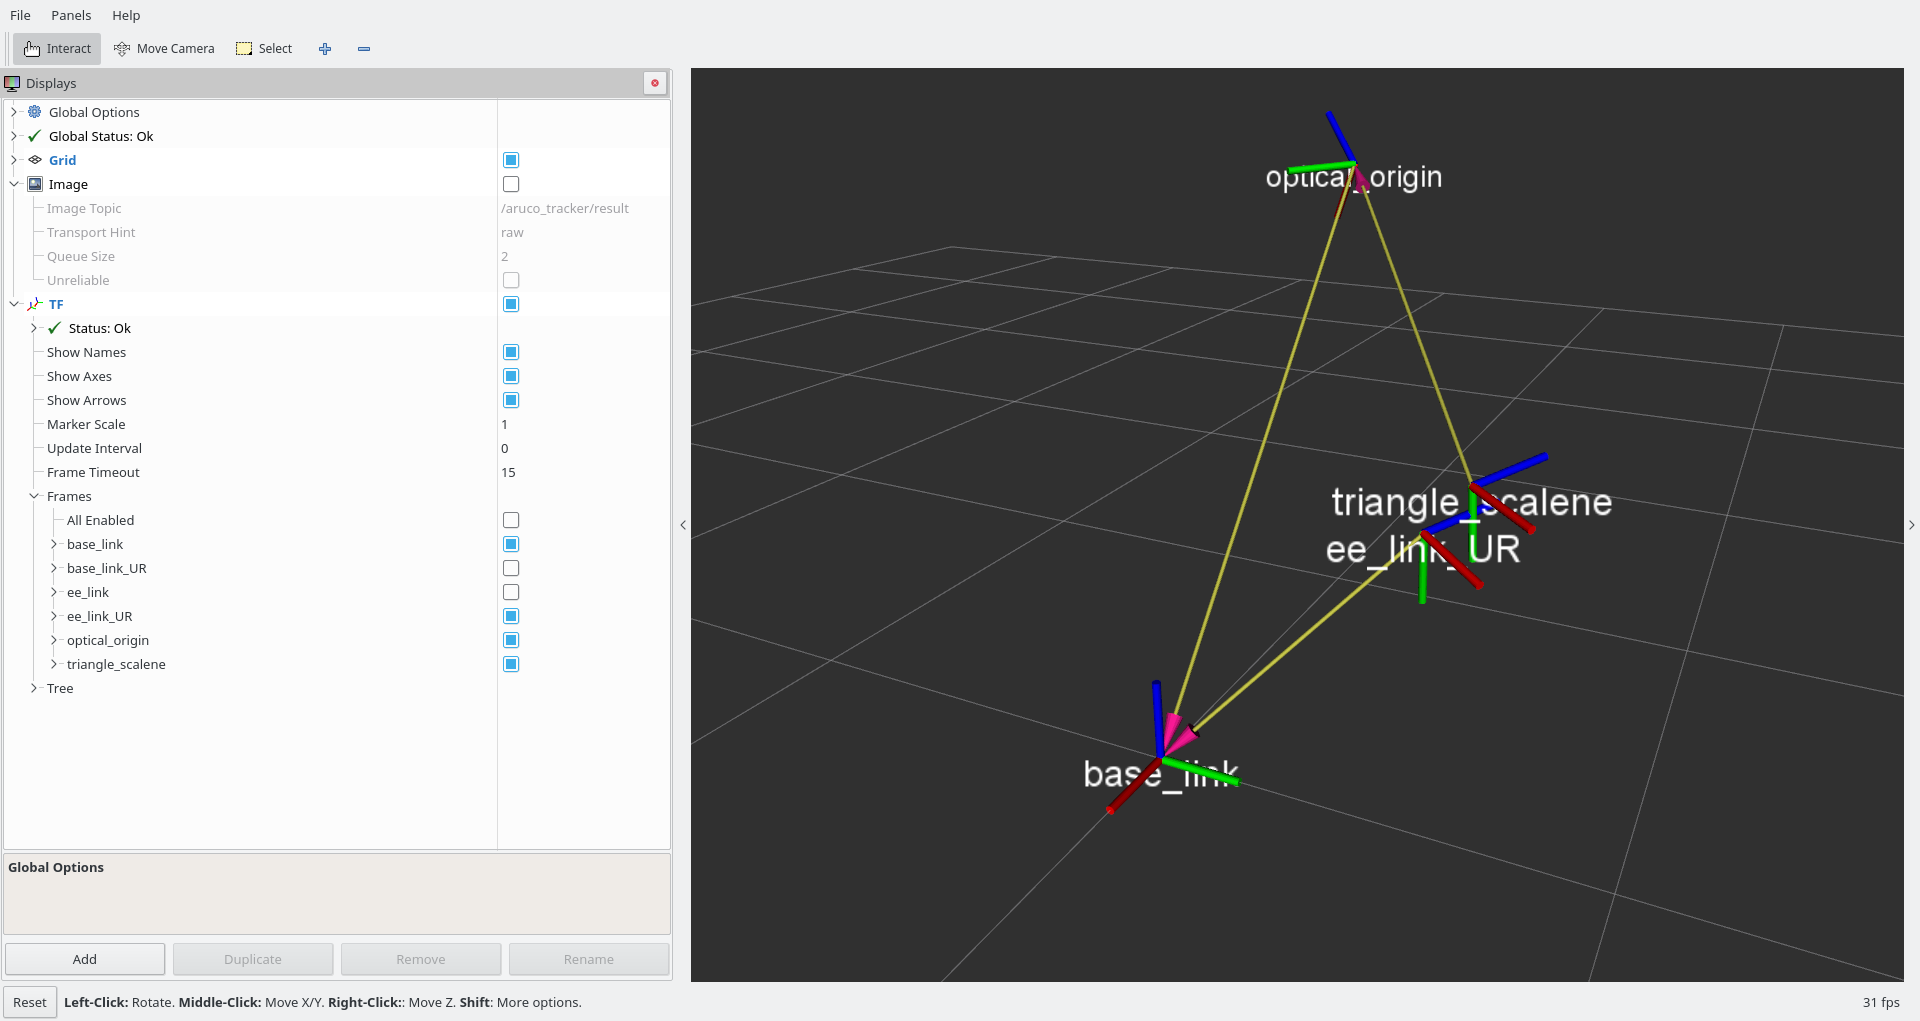
\includegraphics[width=0.7\columnwidth]{figure/设计方案/软件设计/calibrated_rviz.png}
    \caption{使用easy\_handeye进行手眼标定}
\end{figure}

\subsubsection{联合标定}
联合标定是指标定相机坐标系与IMU坐标系的转换关系，进行联合标定的目的同样是为了更精确地估计目标在世界坐标系的位姿，以及云台在世界坐标系的姿态。正如手眼标定中所提到的原因，urdf中相机坐标系与IMU坐标系的转换与实际机器人中的存在误差。借助IMU反馈数据，可以得出IMU坐标系与世界坐标系的相对姿态关系。在进行联合标定后，我们可以通过坐标系变换来得到相机在世界坐标系的姿态。如果又进行了手眼标定，那么就能精确得到相机在世界坐标系的位姿，同时也可更精确地估计目标在世界坐标系的位姿。

我们使用开源软件包 kalibr\cite{camera_imu_calibration:online} 很方便地进行相机与IMU的联合标定。